\documentclass[11pt,a4paper]{article}

\usepackage[margin=1in]{geometry}
\usepackage{amsmath,amssymb,amsthm}
\usepackage{graphicx}
\usepackage{booktabs}
\usepackage[dvipsnames]{xcolor}
\usepackage{hyperref}
\usepackage{microtype}

\hypersetup{colorlinks=true,linkcolor=blue!50!black,urlcolor=blue!50!black,
            citecolor=blue!50!black}

\newtheorem{theorem}{Theorem}
\newtheorem{proposition}[theorem]{Proposition}
\newtheorem{lemma}[theorem]{Lemma}
\theoremstyle{definition}
\newtheorem{definition}[theorem]{Definition}
\newtheorem{remark}[theorem]{Remark}

\newcommand{\N}{\mathbb{N}}
\newcommand{\Z}{\mathbb{Z}}
\newcommand{\diam}{\operatorname{diam}}
\newcommand{\dist}{\operatorname{d}}

\title{\textbf{Shiftfly}\\[0.3em]
\large A shift-routed interconnect for accelerator fabrics beyond pod scale}
\author{Eylon E. Krause}
\date{}

\begin{document}
\maketitle

\begin{abstract}
Google's TPU interconnect spent nine generations as a Cayley graph of an
abelian group---a $k$-ary $n$-cube whose diameter grows as $\Theta(N^{1/n})$---
before TPU~8i replaced it with \emph{Boardfly}, a three-tier fully connected
hierarchy of Dragonfly type with diameter $7$ over $1{,}152$ chips. We first
audit every shipped TPU topology against the Moore bound and show that at
TPU-class radix ($\Delta \approx 7$) a diameter-$7$ graph could in principle
hold $391{,}910$ chips, so Boardfly spends its diameter budget roughly two
orders of magnitude below the ceiling. We then observe that Boardfly's global
tier is \emph{fully connected}, which does not scale: at $400{,}000$ chips a
group would need $12{,}499$ optical links, so a further hierarchy level must be
stacked and diameters add.

We propose \textbf{Shiftfly}: retain Boardfly's cheap local structure and
replace the fully connected global tier with a generalized Kautz digraph
realised on the existing optical circuit switch. At an identical budget of
$40$ optical ports per group, Shiftfly is a flat graph of guaranteed diameter
$\lceil \log_{d} G\rceil$ over $G$ groups, routes without tables by a shift
register, and admits content addressing natively.

Our evaluation is deliberately two-sided. Shiftfly loses at one-pod scale---
Boardfly achieves chip-level diameter $7$ where Shiftfly needs $11$---and wins
beyond it, with lower diameter, lower mean distance and roughly $2.7\times$
better spectral expansion at equal optical cost. The redundancy result is
mostly negative: locality-aware \emph{placement} accounts for the large
majority of the achievable saving on shared content, and it helps both
topologies, leaving Shiftfly's algebraic path-merging worth only a few percent.
We report the metric trap that conceals this, state the failure modes, and
argue that the honest case for Shiftfly is scaling and expansion, not
deduplication.
\end{abstract}

\tableofcontents

%======================================================================
\section{Introduction}

An accelerator interconnect is a graph, and the quantities that matter---worst
case latency, average latency, bandwidth under adversarial traffic, behaviour
under failure---are graph invariants: diameter, mean distance, bisection width
and connectivity. This paper takes that view literally.

Section~\ref{sec:review} catalogues every Google TPU topology as a graph.
Section~\ref{sec:moore} measures each against the Moore bound, which yields the
observation motivating the rest of the work. Section~\ref{sec:objective}
formalises a second objective---the cost of delivering \emph{the same} content
to many endpoints---because agentic inference makes a large fraction of traffic
semantically redundant. Section~\ref{sec:construction} gives the construction,
Section~\ref{sec:theory} its properties with proofs, Section~\ref{sec:eval} the
measurements, and Section~\ref{sec:limits} the ways it is wrong.

The contribution is not the graph family. Kautz digraphs have been known to be
near-optimal for the directed degree--diameter problem since 1968, and
generalized de~Bruijn and Imase--Itoh digraphs have provided arbitrary-order
versions since 1980--81. The contribution is the argument that this family is
the right global tier for an accelerator fabric that already owns a
reconfigurable optical switch, together with an honest measurement of what that
buys and what it does not.

%======================================================================
\section{TPU topologies as graphs}
\label{sec:review}

\begin{definition}[$k$-ary $n$-cube]
Let $k_1,\dots,k_n \ge 2$. The torus $T(k_1,\dots,k_n)$ is the Cayley graph of
$\Z_{k_1}\times\cdots\times\Z_{k_n}$ with generating set
$\{\pm e_1,\dots,\pm e_n\}$.
\end{definition}

\begin{proposition}
$T(k_1,\dots,k_n)$ has $N=\prod_i k_i$ vertices, is $2n$-regular when all
$k_i>2$, and has
\[
  \diam T = \sum_{i=1}^{n}\left\lfloor k_i/2 \right\rfloor .
\]
In particular a cubic torus has $\diam T = \Theta\!\left(N^{1/n}\right)$.
\end{proposition}

\begin{proof}
Distance in a Cayley graph of an abelian group with this generating set is the
sum of per-coordinate cyclic distances, and the cyclic distance in $\Z_k$ is
maximised at $\lfloor k/2\rfloor$; the maximum is attained simultaneously in
every coordinate.
\end{proof}

The exponent $1/n$ with $n=3$ is the worst scaling in common use, and it was
the right choice while the dominant traffic was nearest-neighbour: dense
training stencils and ring all-reduce touch only adjacent chips, so diameter
never appears on the critical path. Mixture-of-experts routing broke the
assumption. All-to-all traffic pays the diameter on every token.

Table~\ref{tab:review} collects the generations. Diameters for torus
generations are analytic; pod shapes for v5p, v7 and v8t are inferred from
published chip counts and are marked accordingly.

\begin{table}[t]
\centering
\small
\begin{tabular}{lrrrl}
\toprule
Generation & Chips & $\Delta$ & $D$ & Structure \\
\midrule
v2 / v3 & 256 / 1{,}024 & 4 & 16 / 32 & Cayley graph of $\Z_k^2$\\
v4 & 4{,}096 & 6 & 24 & $\Z_{16}^3$, $4^3$ cubes, OCS between cubes\\
v5e / v6e & 256 & 4 & 16 & $\Z_{16}^2$\\
v5p & 8{,}960 & 6 & $\approx 32$ & 3D torus (shape inferred)\\
v7 Ironwood & 9{,}216 & 6 & $\approx 32$ & 3D torus; chiplets add a 4th logical axis\\
v8t & 9{,}600 & 6 & $\approx 33$ & 3D torus, Virgo scale-out fabric\\
\textbf{v8i} & \textbf{1{,}152} & \textbf{7} & \textbf{7} & \textbf{Boardfly}: 3-tier fully connected\\
\bottomrule
\end{tabular}
\caption{Google TPU interconnects as graphs.}
\label{tab:review}
\end{table}

\paragraph{Boardfly.} Google describes it as ``a building block of four fully
connected chips into a fully connected group of eight boards, with 36 of such
groups fully connected into a TPU~8i pod''. Thus a building block holds $4$
chips, a group holds $8$ building blocks, i.e.\ $32$ chips, and a pod holds
$36$ groups, i.e.\ $1{,}152$ chips. Each building block exposes $16$ external
links of which $11$ serve the group in copper, leaving $5$ per building block
and hence $40$ optical ports per group. Within a pod the $36$ groups are fully
connected through the optical circuit switch, consuming $35$ of those $40$.

\begin{lemma}[Boardfly's diameter decomposition]
\label{lem:seven}
If the optical link between two groups terminates on one designated chip of one
designated building block on each side, the chip-level pod diameter is $7$.
\end{lemma}

\begin{proof}
Reaching the group's egress chip costs at most three hops: one inside the
source building block, one across the copper link to the building block owning
the optical port, one inside that building block. The optical hop is one. The
destination side is symmetric. Hence $3+1+3=7$, and the bound is attained.
\end{proof}

We adopt Lemma~\ref{lem:seven}'s accounting throughout. Traversing $g$
inter-group hops passes through $g+1$ groups, so

\begin{equation}
\label{eq:chiphops}
  \text{chip hops} \;=\; \iota\,(g+1) + g, \qquad \iota = 3 ,
\end{equation}

which reproduces $7$ at $g=1$. Our chip-level simulation of a Boardfly pod
measures diameter exactly $7$, confirming the port model.

%======================================================================
\section{The Moore-bound audit}
\label{sec:moore}

\begin{theorem}[Moore bound]
A graph of maximum degree $\Delta \ge 3$ and diameter $D$ has
\[
  N \;\le\; 1 + \Delta\sum_{i=0}^{D-1}(\Delta-1)^i
    \;=\; \frac{\Delta(\Delta-1)^{D}-2}{\Delta-2}.
\]
\end{theorem}

\begin{proof}
Fix $v$. Breadth-first from $v$ reaches at most $\Delta$ vertices at distance
$1$ and, since each subsequent vertex has at most $\Delta-1$ unused incident
edges, at most $\Delta(\Delta-1)^{i-1}$ at distance $i$. Every vertex lies
within distance $D$.
\end{proof}

Equality requires a Moore graph, and these exist only for $D=1$, for cycles,
and for $D=2$ with $\Delta\in\{3,7,57\}$. The bound is therefore a ceiling, and
the informative quantity is the ratio to it.

At $\Delta=7$:
\[
  \text{Moore}(7,4)=1{,}814,\quad
  \text{Moore}(7,5)=10{,}886,\quad
  \text{Moore}(7,6)=65{,}318,\quad
  \text{Moore}(7,7)=391{,}910 .
\]

Two consequences. First, Boardfly attains diameter $7$ at $1{,}152$ chips,
whereas $\Delta=7$ permits diameter $4$ at that order---so even at its own
scale the design is about $1.75\times$ off. Second, and more importantly,
$\Delta = 7$ admits diameter $7$ at almost exactly $400{,}000$ chips. Boardfly
therefore spends, at pod scale, the diameter that would in principle serve a
$400{,}000$-chip machine.

\begin{remark}
This is not a claim that a $400{,}000$-chip diameter-$7$ machine is buildable.
Moore-optimal graphs of large diameter are not known, and the bound ignores
bisection, cabling length and fault tolerance---all of which Boardfly is buying
with its slack. It is a claim that the slack is unusually large and worth
interrogating.
\end{remark}

\paragraph{The structural obstruction.} Boardfly's global tier is a complete
graph $K_{36}$ on groups, so a group needs $G-1$ optical ports to reach $G$
groups. With $G=12{,}500$ (i.e.\ $400{,}000$ chips at $32$ chips per group)
this is $12{,}499$ ports against $40$ available. Full connectivity does not
scale; another hierarchy level must be added, and by \eqref{eq:chiphops} each
added level costs four chip hops. This is the weakness Shiftfly attacks.

%======================================================================
\section{Two objectives}
\label{sec:objective}

Latency is the standard objective: minimise $\diam G$ and the mean distance
$\bar{\dist}(G)$. The second objective is specific to agentic inference, where
one user query fans out into many concurrent rollouts that share a system
prompt, tool definitions and retrieved context, and therefore request the
\emph{same} content.

\begin{definition}[Multicast cost]
Let $h$ be the home vertex of a content item and $S$ the set of requesters. The
\emph{unicast cost} is $U(S,h)=\sum_{v\in S}\dist(v,h)$. The \emph{tree cost}
$T(S,h)$ is the number of edges in the union of shortest paths from each $v\in
S$ to $h$, i.e.\ what a fabric with in-network replication pays. The
\emph{multicast efficiency} is $\eta(S,h)=U(S,h)/T(S,h)$.
\end{definition}

\begin{remark}[A metric trap]
\label{rem:trap}
$\eta$ must not be optimised alone. It is a ratio, and a topology is rewarded
for placing requesters \emph{far} from the home vertex provided their paths
overlap. A network in which everything is one hop away scores $\eta=1$---the
worst possible value---while paying the least. Our measurements exhibit exactly
this inversion: Boardfly attains higher $\eta$ than Shiftfly while paying
higher absolute $T$. The quantity to minimise is $T$; $\eta$ is diagnostic
only.
\end{remark}

The design problem is the bi-objective
\begin{equation}
\label{eq:biobj}
  \min_{G:\ \Delta(G)\le\Delta_{\max}}
  \Bigl(\ \bar{\dist}(G),\ \ \mathbb{E}_{S,h}\bigl[T(S,h)\bigr]\ \Bigr),
\end{equation}
and the two conflict. Expander graphs minimise $\bar{\dist}$ but random routes
share few edges; trees maximise sharing and have poor diameter and bisection.

%======================================================================
\section{The construction}
\label{sec:construction}

\begin{definition}[Kautz digraph]
For $d\ge2$ and $D\ge1$, $K(d,D)$ has as vertices the words
$u_1u_2\cdots u_D$ over an alphabet of size $d+1$ with $u_i\neq u_{i+1}$, and
an arc $u \to u_2\cdots u_D\alpha$ for every $\alpha \neq u_D$.
\end{definition}

\begin{definition}[Shiftfly]
Retain Boardfly's building block ($4$ chips, complete) and group ($8$ building
blocks, complete; $32$ chips). Replace the complete global tier by a Kautz
digraph on the groups, realised as a fixed permutation installed on the optical
circuit switch. When the group count is not of the form $(d+1)d^{D-1}$, use the
Imase--Itoh digraph on $\Z_n$ with arcs $i \mapsto -di-r \bmod n$,
$r=1,\dots,d$, which exists for every $n$.
\end{definition}

\begin{remark}[Port accounting]
\label{rem:ports}
In $K(d,D)$ a vertex $u$ is both a successor and a predecessor of $v$ exactly
when $u_1 = u_D$, and then in exactly one neighbour: solving
$u_2\cdots u_D\alpha = \beta u_1 \cdots u_{D-1}$ forces $\beta = u_2$,
$u_1 = u_D$ and $\alpha = u_2$. There are $d(d+1)$ such vertices out of
$(d+1)d^{D-1}$, a fraction $d^{2-D}$. Undirected degree is therefore $2d$, or
$2d-1$ on that thin set, so \textbf{out-degree $d$ costs $2d$ bidirectional
ports}. Matching Boardfly's $40$ optical ports per group means $d=20$, not
$d=40$; comparing at $d=40$ silently doubles Shiftfly's hardware and
invalidates the result. We report only $d=20$, and the simulator asserts the
edge counts of the two designs agree to within $5\%$.
\end{remark}

%======================================================================
\section{Properties}
\label{sec:theory}

\begin{theorem}[Order, degree, diameter]
\label{thm:kautz}
$K(d,D)$ has $N=(d+1)d^{D-1}$ vertices, out-degree and in-degree $d$, and
diameter exactly $D$.
\end{theorem}

\begin{proof}
There are $d+1$ choices for $u_1$ and $d$ for each subsequent symbol, giving
the order. Out-degree is the number of $\alpha \neq u_D$, namely $d$. For the
diameter, given $u$ and $v$ the word $u_{k+1}\cdots u_D v_1 \cdots v_k$ is a
legal vertex whenever the junction symbols differ, and applying the arc map $D$
times transforms $u$ into $v$; hence $\dist(u,v)\le D$. It is exactly $D$ for
$u,v$ sharing no admissible overlap.
\end{proof}

Against the directed Moore bound $N \le (d^{D+1}-1)/(d-1)$, $K(d,D)$ is within
a factor $1+O(1/d)$: it is essentially optimal among digraphs.

\begin{theorem}[Shift routing]
\label{thm:shift}
For $u,v \in K(d,D)$ the sequence
$w^{(k)} = u_{k+1}\cdots u_D v_1\cdots v_k$, $k=0,\dots,D$, is a walk from $u$
to $v$ of length at most $D$, computable from the labels alone.
\end{theorem}

\begin{proof}
$w^{(0)}=u$ and $w^{(D)}=v$, and $w^{(k+1)}$ is obtained from $w^{(k)}$ by
deleting the leading symbol and appending $v_{k+1}$, which is the arc map.
\end{proof}

Theorem~\ref{thm:shift} is the operational point: routing requires no tables,
no routing protocol and no convergence, at any scale. The destination label is
the route.

\begin{theorem}[Merge criterion]
\label{thm:merge}
Let $u,u'$ route to a common $v$ under Theorem~\ref{thm:shift}. Their walks
occupy the same vertex at step $k$ if and only if $u$ and $u'$ agree in their
last $D-k$ symbols. Consequently the first merge occurs at
\[
  k^{*}(u,u') \;=\; D - \operatorname{lcs}(u,u'),
\]
where $\operatorname{lcs}$ is the length of the longest common suffix.
\end{theorem}

\begin{proof}
By Theorem~\ref{thm:shift}, $w^{(k)}$ depends on $u$ only through
$u_{k+1}\cdots u_D$ and on $v$ through a prefix common to both walks. Equality
of $w^{(k)}$ and $w'^{(k)}$ is therefore equivalent to equality of those
suffixes.
\end{proof}

Theorem~\ref{thm:merge} says redundant requests collapse \emph{structurally}:
once two requests for the same item meet, the second can be served from an
in-network cache at the meeting point, with no coordination, no directory and
no protocol. It is a statement about the routing algebra.

\begin{proposition}[Random labels give almost no merging]
\label{prop:random}
If labels are assigned uniformly at random, then
$\Pr[\operatorname{lcs}(u,u')\ge j] = d^{-j}(1+o(1))$, so
$\mathbb{E}[\operatorname{lcs}] = \frac{1}{d-1}(1+o(1))$ and
$\mathbb{E}[k^{*}] = D - \frac{1}{d-1}(1+o(1))$.
\end{proposition}

\begin{proof}
Symbols are independent given the no-repeat constraint, and each successive
suffix symbol agrees with probability $1/d$ up to the constraint correction.
\end{proof}

At $d=20$ this is $\mathbb{E}[\operatorname{lcs}]\approx 0.053$: essentially no
merging before the destination. \textbf{The merge property is not free.} It is
purchased by choosing the labelling so that groups likely to want the same
content are suffix-close---and that is the co-design step, an embedding of the
observed sharing hypergraph into the suffix tree.

\begin{theorem}[Arbitrary order]
The Imase--Itoh digraph on $\Z_n$ with arcs $i\mapsto -di-r \bmod n$,
$r=1,\dots,d$, has out-degree $d$ and diameter at most $\lceil \log_d n\rceil$
for every $n\ge2$.
\end{theorem}

\begin{proof}[Proof sketch]
Iterating the arc map $k$ times sends $i$ to $(-d)^k i - \sum_{j} r_j (-d)^{k-j}
\bmod n$. As the $r_j$ range over $\{1,\dots,d\}$ the reachable set after $k$
steps has size $\min(d^k, n)$, and covers $\Z_n$ once $d^k \ge n$.
\end{proof}

This removes the quantisation that would otherwise strand capacity: a Kautz
graph exists only at orders $(d+1)d^{D-1}$, and a real machine is whatever size
it is.

\begin{proposition}[Connectivity]
$K(d,D)$ has vertex connectivity $d$, the maximum possible at that degree.
\end{proposition}

Thin global tiers are the usual fragility of hierarchical fabrics; maximal
connectivity is the relevant defence.

%======================================================================
\section{Evaluation}
\label{sec:eval}

All measurements come from the accompanying simulator, which is
dependency-free and reproduces every table and figure from one script.
Distances are exact by breadth-first search where the instance permits and
sampled otherwise, and sampled figures are labelled as such. Spectral gaps are
power-iteration estimates. Both designs receive $40$ optical ports per group
and identical $32$-chip group internals, so the comparison is at matched
optical cost (Remark~\ref{rem:ports}).

\subsection{Model validation}
The chip-level Boardfly pod model has $1{,}152$ vertices, maximum degree $7$,
and \textbf{measured diameter exactly $7$}, matching the published figure and
Lemma~\ref{lem:seven}.

\subsection{Scaling}
Figure~\ref{fig:diam} reports chip-level diameter against system size.
\textbf{Boardfly wins at one-pod scale} ($7$ against Shiftfly's $11$ at
$1{,}152$ chips) and loses beyond it, because the complete global tier must be
re-hierarchised while the Kautz tier merely grows one symbol. Mean distance and
spectral expansion follow the same pattern; at the scales tested Shiftfly's
spectral gap is roughly $2.7\times$ Boardfly's, which is unsurprising in
hindsight: a hierarchy of near-cliques joined by few links is a poor expander
by construction, whatever its diameter.

\begin{figure}[t]
\centering
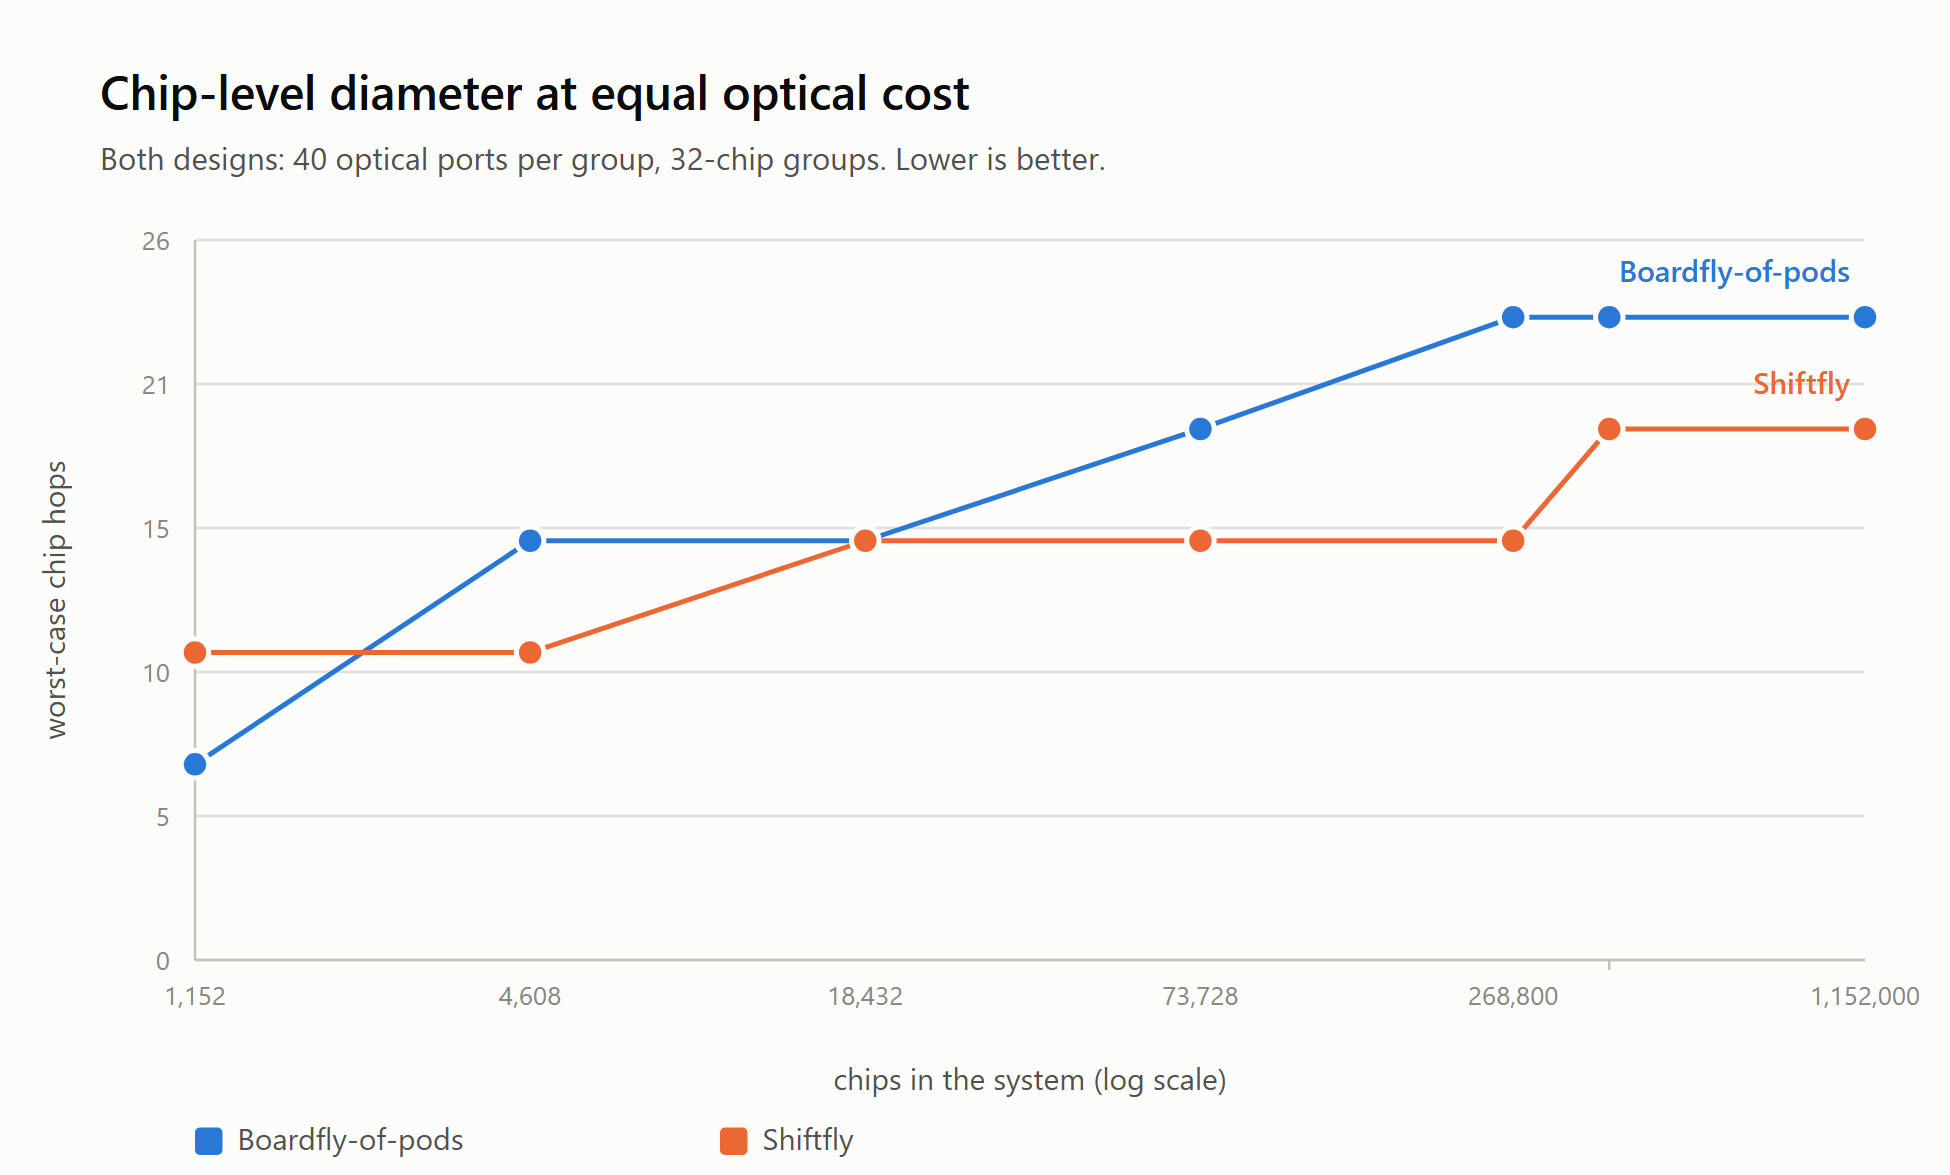
\includegraphics[width=0.92\textwidth]{../figures/diameter_vs_scale.png}
\caption{Chip-level worst-case distance at equal optical cost. Boardfly is
better at pod scale; the crossing is the result.}
\label{fig:diam}
\end{figure}

\begin{figure}[t]
\centering
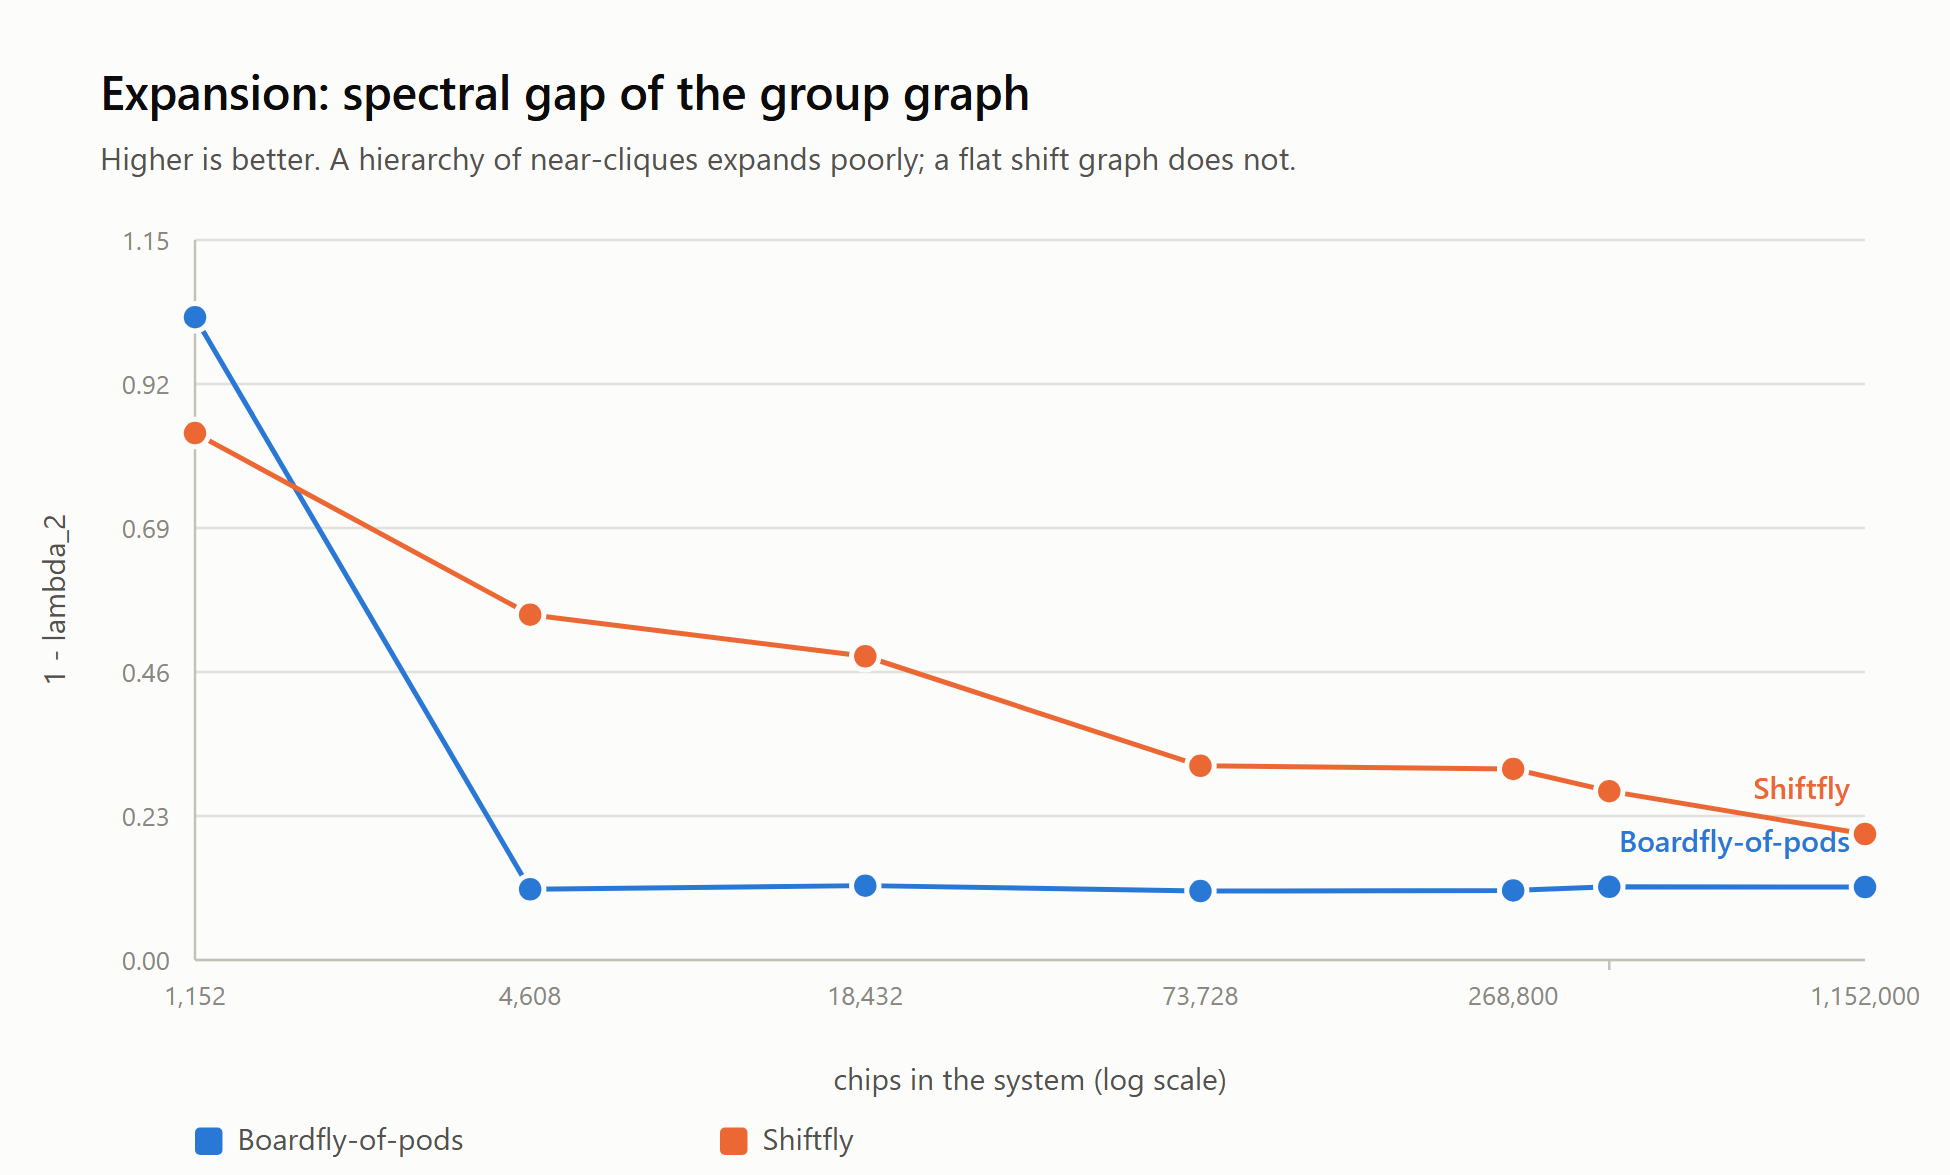
\includegraphics[width=0.92\textwidth]{../figures/spectral_gap.png}
\caption{Spectral gap of the group graph. A hierarchy of near-cliques joined
by few links expands poorly whatever its diameter; the flat shift graph does
not.}
\label{fig:gap}
\end{figure}

\subsection{Scaling: the numbers}
At matched optical cost, chip-level worst-case distance is:

\begin{center}
\small
\begin{tabular}{rrr}
\toprule
Chips & Boardfly & Shiftfly \\
\midrule
1{,}152 & \textbf{7} & 11 \\
4{,}608 & 15 & \textbf{11} \\
18{,}432 & 15 & 15 \\
73{,}728 & 19 & \textbf{15} \\
268{,}800 & 23 & \textbf{15} \\
400{,}000 & 23 & \textbf{19} \\
1{,}152{,}000 & 23 & \textbf{19} \\
\bottomrule
\end{tabular}
\end{center}

At the $400{,}000$-chip target the reduction is $23 \to 19$, or $17\%$; the
largest gap in the sweep is $23 \to 15$ at $268{,}800$ chips, where Boardfly has
just paid for another hierarchy level and Shiftfly has not yet needed another
symbol. Both curves are step functions, so the advantage is not monotone.

\subsection{Sharing}
This is where the proposal is weakest, and we state it plainly. Writing $T$ for
tree hops per requester:

\begin{center}
\small
\begin{tabular}{lrrrr}
\toprule
& \multicolumn{2}{c}{$T$ (lower is better)} & \multicolumn{2}{c}{merge depth}\\
\cmidrule(lr){2-3}\cmidrule(lr){4-5}
Placement & Boardfly & Shiftfly & Boardfly & Shiftfly\\
\midrule
random           & 2.768 & 2.470 & 2.868 & 2.772 \\
locality-aware   & 2.174 & \textbf{2.112} & 2.336 & \textbf{2.152} \\
\midrule
saving from placement & $-21.5\%$ & $-14.5\%$ & & \\
\bottomrule
\end{tabular}
\end{center}

Locality-aware placement removes $21.5\%$ of tree cost on Boardfly and $14.5\%$
on Shiftfly. \textbf{Shiftfly's residual advantage at matched placement is
$2.9\%$}, with merge depth $7.9\%$ lower. The overwhelming majority of the
available saving on shared content therefore comes from \emph{placement}, which
is topology-agnostic, and not from the shift algebra.

Furthermore the efficiency ratio $\eta$ ranks Boardfly \emph{higher}
($1.431$ against $1.364$) while absolute tree cost ranks it \emph{lower}
($2.174$ against $2.112$)---precisely the inversion predicted in
Remark~\ref{rem:trap}. Had we reported $\eta$ alone, as the natural reading of
the objective in \eqref{eq:biobj} invites, we would have drawn the opposite
conclusion.

\paragraph{Conclusion of the evaluation.} The defensible case for Shiftfly is
scaling and expansion. The redundancy case, as measured here, is
\emph{primarily an argument for locality-aware placement}, which is
topology-agnostic.

%======================================================================
\section{Limitations, and how this could be wrong}
\label{sec:limits}

\begin{enumerate}
\item \textbf{Boardfly is better at the scale it was designed for.} At
$1{,}152$ chips the complete global tier is simply the right answer. Nothing
here contradicts that choice.

\item \textbf{Bisection.} De~Bruijn and Kautz families have bisection width
$\Theta(N/\log N)$, against $\Theta(N)$ for a complete or expander tier.
Measured against a \emph{hierarchy} the comparison favours Shiftfly, because
hierarchies expand badly; measured against a flat high-radix fabric it would
not. All-to-all-dominated workloads are the adversarial case.

\item \textbf{Cabling.} Shift edges are long and irregular, which is the
standard reason de~Bruijn networks are not built. The mitigation is specific
and not general: the global tier is already optically circuit-switched, so the
wiring is a permutation the switch installs, not copper anyone routes. This
argument is available to an operator that owns an OCS layer and to essentially
nobody else.

\item \textbf{Deterministic routing.} Shift routing yields one path. Load
balance will require non-minimal alternatives, and randomising the route partly
destroys the merge property of Theorem~\ref{thm:merge}. The interaction is
unquantified here.

\item \textbf{The switch is mechanical.} MEMS-based optical circuit switches
reconfigure in milliseconds to seconds, so the Kautz permutation is fixed at
scheduling time. Label assignment is therefore a scheduling decision, not a
runtime one.

\item \textbf{The workload model is synthetic.} Cluster count, agent fan-out,
scheduler locality and Zipf exponent are chosen to be plausible, not measured.
The sharing conclusions are only as good as those four numbers.
\end{enumerate}

%======================================================================
\section{Related work}

Dragonfly established the high-radix hierarchical form that Boardfly follows.
The degree--diameter literature supplies the ceiling used in
Section~\ref{sec:moore}, and recent topologies---Slim~Fly from
McKay--Miller--\v{S}ir\'a\v{n} graphs, PolarFly from Erd\H{o}s--R\'enyi
polarity graphs, Bundlefly---pursue it directly at router radix. Shiftfly
differs in operating at accelerator radix, where the endpoint \emph{is} the
router, and in taking the content-addressing property of the shift families
seriously; the same algebra underlies the Koorde distributed hash table.
Kautz digraphs are due to Kautz; the arbitrary-order generalizations to Reddy,
Pradhan and Kuhl, and to Imase and Itoh.

%======================================================================
\section{Conclusion}

Google's move from torus to Boardfly traded a $\Theta(N^{1/3})$ diameter for a
constant one and was clearly correct for a $1{,}152$-chip inference pod. The
mechanism it used---full connectivity at every tier---does not extend, because
complete graphs need $N-1$ ports. Replacing only the global tier with a
generalized Kautz digraph keeps the diameter logarithmic in the number of
groups at a fixed port budget, yields table-free routing and native content
addressing, and measurably improves expansion.

The redundancy argument that motivated the design did not survive its own
evaluation intact: most of the available saving on shared content comes from
placement, not from topology. We regard reporting that as more useful than
the alternative.

\appendix
\section{Reproduction}
\begin{verbatim}
git clone https://github.com/EylonKrause/shiftfly
cd shiftfly
python3 run_experiments.py           # stdlib only
python3 -m unittest discover -s tests
\end{verbatim}

\end{document}
